%%%%%%%%%%%%%%%%%%%%%%%%%%%%%%%%%%%%%%%%%%%%%%%%%%%%
\documentclass[10pt]{article}
%%%%%%%%%%%%%%%%%%%%%%%%%%%%%%%%%%%%%%%%%%%%%%%%%%%%

% Loading of symbols libraries
\usepackage{fullpage}     % To get full-page documments
\usepackage{amsmath}
\usepackage{latexsym}
\usepackage{amssymb}
\usepackage{psfrag}       % Replace utility in pictures
\usepackage{graphicx}     % \includegraphics[]{}
\usepackage{subfigure}
\usepackage{times} 	
\usepackage{xspace}	
\usepackage{url}	



\title{\textbf{\PDT-\JACK\ Basic Agent System for the Gold Mining Game} \\
User Manual}
\author{Sebastian Sardina \\ Version 2.5}
% \date{}


\pagenumbering{arabic}
\renewcommand{\baselinestretch}{1}    % Spacing.

%%%%%%%%%%%%%%%%%%%%%%%%%%%%%%%%%%%
% User defined macros - START 
%%%%%%%%%%%%%%%%%%%%%%%%%%%%%%%%%%%
%\input{Psfig}               % Include PS macros for including PS-EPS

%% PROPER NAMES: Golog, ConGolog, CAN, AgentSpeak, etc...
\newcommand{\propername}[1]{\mbox{\sf #1}\xspace}
\newcommand{\propernamesmall}[1]{\mbox{\small \sf #1}}
\newcommand{\propernametiny}[1]{\mbox{\tiny \sf #1}}
% \newcommand{\propername}[1]{\textsc{\sc #1}}
\newcommand{\Golog}{\propername{Golog}}
\newcommand{\GologSpeak}{\propername{GologSpeak}}
\newcommand{\DGolog}{\propername{DGolog}}
\newcommand{\sGolog}{\propername{sGolog}}
\newcommand{\ConGolog}{\propername{ConGolog}}
\newcommand{\IndiGolog}{\propername{IndiGolog}}
\newcommand{\LeGolog}{\propername{LeGolog}}
\newcommand{\DTGolog}{\propername{DTGolog}}
\newcommand{\Prolog}{\propername{Prolog}}
\newcommand{\AgentSpeak}{\propername{AgentSpeak}}
\newcommand{\JASON}{\propername{Jason}}
\newcommand{\CANMINUS}{\propername{Can$^{\cal C}$}}
\newcommand{\CANMINUST}{\propernametiny{Can$^{\cal C}$}}
\newcommand{\CAN}{\propername{Can}}
\newcommand{\CANT}{\propernametiny{Can}}
\newcommand{\CANPLAN}{\propername{CanPlan}}
\newcommand{\CANPLANT}{\propernametiny{CanPlan}}
\newcommand{\CANPLANII}{\propername{CanPlan2}}
\newcommand{\CANPLANOR}{\propername{Can(Plan)}}
\newcommand{\JACK}{\propername{Jack}}
\newcommand{\PDT}{\propername{PDT}}
\newcommand{\ECLIPSE}{\propername{ECLIPSe}}
\newcommand{\JDE}{\propername{JDE}}
\newcommand{\JACKTM}{\propername{Jack\texttrademark}}
\newcommand{\JAM}{\propername{JAM}}
\newcommand{\PRS}{\propername{PRS}}
\newcommand{\RAP}{\propername{Rap}}
\newcommand{\dMARS}{\propername{dMARS}}
\newcommand{\TAPL}{\propername{3APL}}
\newcommand{\JSHOP}{\propername{JShop}}
\newcommand{\SHOP}{\propername{Shop}}
\newcommand{\SHOPII}{\propername{Shop2}}
\newcommand{\Retsina}{\propername{Retsina}}
\newcommand{\IPEM}{\propername{Ipem}}
\newcommand{\SAGE}{\propername{Sage}}
\newcommand{\DECAF}{\propername{Decaf}}
\newcommand{\PROPICE}{\propername{Propice-Plan}}
\newcommand{\CYPRESS}{\propername{Cypress}}
\newcommand{\CPEF}{\propername{Cpef}}


\newcounter{bean}

\newenvironment{tightenumerate}{
                \begin{list}{
                  {\mbox {
                      \arabic{bean}.\/}}}{\usecounter{bean}
                      \setlength{\itemsep}{-3pt}\setlength{\topsep}{0pt}}}{
                \end{list}}

\newenvironment{tightitemize}{
                \begin{list}{$\bullet$}{
                    \setlength{\itemsep}{-3pt}}{\setlength{\topsep}{0pt}}}{
                \end{list}}
%\setlength{\itemsep}{0pt}}{\setlength{\topsep}{0pt}}}{

%%%%%%%%%%%%%%%%%%%%%%%%%%%%%%%%%%%
% User defined macros - END 
%%%%%%%%%%%%%%%%%%%%%%%%%%%%%%%%%%%


\begin{document}

\maketitle               % Title Generation
%\tableofcontents        % Index Generation
%\pagebreak
%\thispagestyle{empty}   % No numbering for this titule page



This document briefly describes the \JACK\ \textit{core} agent framework for the gold mining game. This is a basic agent framework to serve as an initial system to build on more sophisticated systems.

On of the most important aspect of this framework is its support infrastructure implementing the ``glue'' between the player agents and the game server. Therefore, the framework already encapsulates all the connectivity code required to communicate with the game server.
%
Besides this, the system also includes some very basic (random) agent behaviour too, as some useful code that could be used as examples for further extensions.

The design of the system was done using the \PDT tool (as an \ECLIPSE plugin), but substantial \JACK\ coding was also done on the \JACK\ sources to provide a basic behavior. When re-generating code, \PDT\ will respect the added code.



\subsection*{Disclaimer}

The current document should be treated as ``informal'' notes aimed to quickly help the user to understand the system and use it. Nevertheless, this document is far from complete and checked and has suffered many changes since its original version. Therefore, the reader should be aware that there may be many errors and inconsistencies.


%%%%%%%%%%%%%%%%%%%%%%%%%%%%%%%%%%%%%%%%%%%%%%%%%%%%
\section{File System Structure}
%%%%%%%%%%%%%%%%%%%%%%%%%%%%%%%%%%%%%%%%%%%%%%%%%%%%

The system file and directory structure is as follows:
\begin{description}

\item[\rm \texttt{README.TXT}] Short instructions on how to run the application.

\item[\rm \texttt{FILES.TXT}] Description of file/directory contents in the application.

\item[\rm \texttt{design.pd}] The \PDT\ file containing the agent system design. 

\item[\rm \texttt{run-team.sh}] Shell script to \textit{run} the agent system application. 

\item[\rm \texttt{Makefile}]  Makefile for clean (\texttt{make clean}), compile (\texttt{make compile}), and pack the application into a JAR file (\texttt{make jar}). To do everything (i.e., clean-compile-pack) one can use \texttt{make all}.

\item[\rm \texttt{compile.sh}] Shell script to \textit{compile} the \JACK\ application. This script will	take the	\JACK\ source code and compile it using both Java	compiler and \JACK\ kernel. Binaries will be placed in \texttt{bin/} and a whole JAR \texttt{jackagt.jar} file will be placed in \texttt{lib/}.

\item[\rm \texttt{build-jack.xml}] Ant script to \textit{compile} the \JACK\ application within \ECLIPSE.


 \item[\rm \texttt{lib/}] Location where all the required libraries, as JAR files, should be placed, including \texttt{jack.jar} containing the \JACK compiler and runtime environment and \texttt{gui.jar} containing the GUI interface. These libraries are used both at development time (when designing and compiling the application) as well as execution time (when running the application itself).
 
\item[\rm \texttt{src/}]   The location for all sources for the application, including the \JACK\ sources. In particular, \PDT\ will generate \JACK\ code in subdirectory \texttt{src/rmit/ai/clima/jackagt/}.


\item[\rm \texttt{bin/}]  The location where the \JACK\ \textit{binary} application will be placed when the \JACK\ source is compiled. It will also contain the corresponding \texttt{.java} files generating by \JACK\ compiler.

\end{description}


%%%%%%%%%%%%%%%%%%%%%%%%%%%%%%%%%%%%%%%%%%%%%%%%%%%%
\section{Mini How-To}
%%%%%%%%%%%%%%%%%%%%%%%%%%%%%%%%%%%%%%%%%%%%%%%%%%%%
% 
To set up your system you should first follow these initial steps:
%
\begin{enumerate}\addtolength{\itemsep}{-.02in}
  
 \item Make sure JDK 1.6 is installed in the system. JRE is not sufficient as we will need to \textit{compile} the JAVA code generated by \JACK. JDK can be easily obtained from Sun web-page at \texttt{http://java.sun.com/}. 

\item Make sure you have lastest \ECLIPSE installed in your system.
 
\item Install the \PDT plugin for \ECLIPSE.
\begin{itemize}
  \item If you use Windows and do not have administration rights (e.g., at RMIT lab), follow the instructions at:
  	\begin{center}
  		\url{http://yallara.cs.rmit.edu.au/~hosun/PDTWWW/pdt_rmit_lab_install.html}
  	\end{center}

  \item If you use Windows and have administration rights, follow the instructions at:

  	\begin{center}
		\url{	http://code.google.com/p/pdt-plugin/wiki/QuickStartManual}
  	\end{center}
		
  	
  	\item If you use Linux, then just copy the two \PDT JAR files to your \texttt{$\sim$/.eclipse} plugin subdir.
  
\end{itemize}


\item Get the basic \JACK\ agent system and unpack it as a new \ECLIPSE project.

\item Get and install JAR files \texttt{jack.jar}, \texttt{climacomms.jar}, and \texttt{gui.jar}, into the \texttt{lib/} sub-directory of your agent system.

\item Get the game server package \texttt{game-server-AOPD0X.zip} and unpack it. Read its \texttt{readme.txt} file and configure the ports to be used.

\end{enumerate}


Once you set-up both the server and the agent systems, you will generally follow these steps to update and run the agent system:
%
\begin{enumerate}\addtolength{\itemsep}{-.02in}
\item Open \PDT  file \texttt{design.pd} from inside \ECLIPSE.

\item Using \PDT, implement the desired \textit{design} changes/extensions required for your system (e.g., add a new entity or link two entities).

\item Instruct \PDT\ to generate all \JACK\ source code files in source directory \texttt{src/rmit/ai/clima/jackagt}. \PDT\ will
generate the corresponding \texttt{.agent}, \texttt{.cap}, \texttt{.bel}, \texttt{.event}, \texttt{.plan} files in corresponding sub-directories. Remember to set-up both the source directory \texttt{src/} and the package \texttt{rmit.ai.clima.jackagt} correctly; you only need to do this the firs time you generate code, \PDT will remember both options.

\item Using the editor of your choice (e.g., \ECLIPSE), implement all  the required code modifications in the \JACK\ source files (e.g., programming code in the body of a plan, or programming the available queries in a new beliefset or the posting methods for an new event). Do all your programming \textit{outside} the \PDT\ protected block, as this will be overwritten by
\PDT\ the next time its code generation facility is used. \PDT, however, will respect all the programming changes you do outside the protected area.


\item Next you must compile the \JACK\ source files to produce the actual executable agent system. This can be done by just running \texttt{make all} in the project main directory, or running script \texttt{compile.sh}. 


\item The (binary) \JACK\ agent system should now be in directory \texttt{bin/} and the whole JAR file \texttt{jackagt.jar} should now be in \texttt{lib/} and ready to be run!

\item Finally, adjust the \texttt{run-team.sh} script to match the server location and the team \textit{usernames} and \textit{passwords}, and run the script to connect to the game server. (If you are running the game server yourself, remember to run the game server \textit{before} the agent system or otherwise the agents will fail to connect.)
\end{enumerate}


For more details on how to \textit{run} the system and options to pass to the \texttt{run-team.sh} script, read file \texttt{readme.txt}.


%%%%%%%%%%%%%%%%%%%%%%%%%%%%%%%%%%%%%%%%%%%%%%%%%%%%
\section{System Components}
%%%%%%%%%%%%%%%%%%%%%%%%%%%%%%%%%%%%%%%%%%%%%%%%%%%%

The system is composed of three agent types: \texttt{Player}, \texttt{Coordinator}, and \texttt{GUIAgent}. 
%
The last agent is responsible of showing the simulation in a graphical window online and to re-play saved simulation afterwards. Here, we shall focus only on the first two agents which are the ones playing the actual game.

A \texttt{Player} agent is an agent acting in the actual game simulator; whereas a \texttt{Coordinator} is an extra agent and does not interact with the game server. Typically, the application will run several player agents (6, in particular) and one coordinator agent.

Within each cycle of a simulation game, the players merely move randomly in the grid, update their current beliefs, and send some information to the coordinator. Meanwhile, the coordinator keeps track of the information received from the players (at this point, very little).
%
Below, we first go over the components within a player agent and then review the ones for the coordinator agent.

\subsection{Player components}

Figure \ref{fig:player-design} depicts the overall design of a player agent.

\begin{figure}
\begin{center}
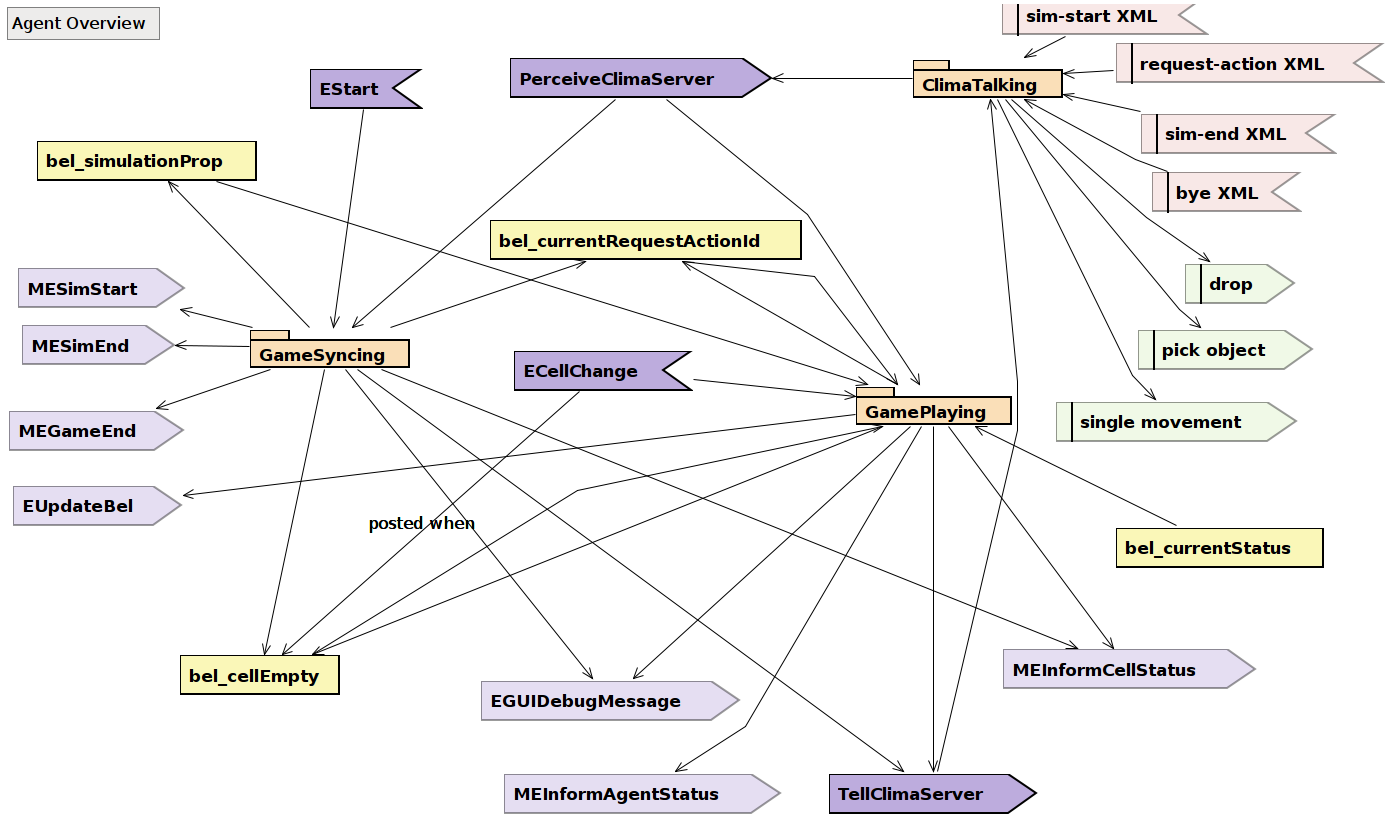
\includegraphics[scale=0.35]{player-design}
\end{center}
\caption{The overall design of a \texttt{Player} agent.}
\label{fig:player-design}
\end{figure}



\subsubsection*{Capabilities}

For modularity, a \texttt{Player} agent is organised into four capabilities:
\begin{description}
 \item[\rm \texttt{ClimaTalking}] All the functionality required for
communication with the game server. This is an external capability (that is,
it is not specified within the system); see Section \ref{sec:clima-talking}.

 \item[\rm \texttt{GameSyncing}] All the functionality required for starting
and ending game simulations and tournaments.

 \item[\rm \texttt{GamePlaying}] All the functionality required for
actually playing a simulation game.

 \item[\rm \texttt{InfoReporting}] All the functionality for displaying
information (e.g., in the console or the GUI window).

\end{description}



% Every player agent has the following beliefs:
%
\subsubsection*{Beliefs}
\begin{itemize}
\item \texttt{CellEmpty}: keep track of which cells are known to have obstacles.

\item \texttt{SimulationProp}: stores some properties of the current simulation
being played.

\item \texttt{LastActionSent}: stores the ID number of the last action sent to
the game server (provided by the \texttt{ClimaTalking} capability).

\item \texttt{CurrentRequestActionId}: stores the ID of the last
\texttt{request-action} message received from the game server.
\end{itemize}


% Figure \ref{fig:design_beliefs} shows the beliefsets of players agents, as
% well as those of the coordinator (see below).



% \begin{figure}
% \begin{center}
% 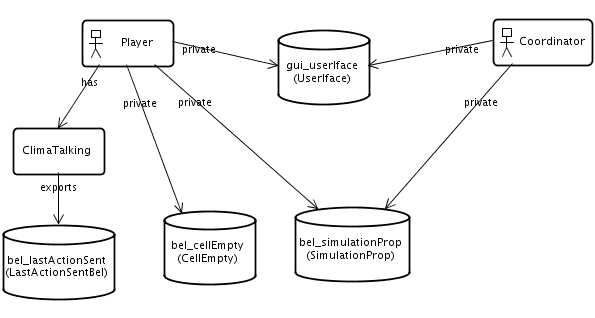
\includegraphics[width=12cm]{BeliefDesign}
% \end{center}
% \caption{An overview of the beliefs used by the application.}
% \label{fig:design_beliefs}
% \end{figure}





\subsubsection*{Events}
\begin{itemize}
\item \texttt{EStart}: signal that the agent has just been created.

\item \texttt{MESimStart} and \texttt{MESimEnd}: message events used to inform
other agents (e.g., the coordinator) of the start and end of simulations,
respectively.

\item \texttt{MEGameEnd}: message event used to inform other agents (e.g.,
the coordinator) of the end of the whole tournament.

\item \texttt{ECellChange}: signals the fac that the beliefs of a cell has changed (e.g., it is now known to be empty of obstacles).

\item \texttt{EAct}: instructs the need to act in the game server (i.e., do an
action).

\item \texttt{EShowBeliefs}: instructs the agent to report on some or all of
what the agent currently believes.

\item \texttt{EExecuteCLIMAaction}: instructs the execution of a particular
domain action (e.g., up or pick).

\item \texttt{TellClimaServer} and \texttt{PerceiveClimaServer}: send and
receive messages to and from the game server, respectively. Both
are provided by the \texttt{ClimaTalking} capability, see Section
\ref{sec:clima-talking}.

\item \texttt{EUpdateBel}: used to trigger the update the beliefs about cells
around a particular location.

\item \texttt{MEInformAgentStatus}: message used to communicate the state of the agent (e.g., its current position to the \texttt{GUIAgent}).

\item \texttt{MEInformCellStatus}: message used to communicate the state of a cell (e.g., inform the \texttt{GUIAgent} that a cell contains an obstacle).
\end{itemize}



\subsubsection*{Plans}
\begin{itemize}
\item \texttt{AuthenticateToServer}: sends the login information to the GAME server by appealing to the \texttt{ClimaTalking} capability.

\item \texttt{StartSimulation} and \texttt{FinishSimulation}: perform tasks associated to the start and end of simulations.

\item \texttt{FinishGame}: perform tasks associated to the end of a complete tournament game.

\item \texttt{HandlePercept}: absorbs all the information encoded in a \texttt{request-action} message from the game server, and then instructs an agent to do something (by posting an event \texttt{EAct}).

\item \texttt{MoveRandomly}: perform some random movement on the grid.

\item \texttt{SendActionAndWait}: sends an action to the game server, by appealing to the \texttt{ClimaTalking} capability.

\item \texttt{BeliefReporting} and \texttt{ConsoleBeliefReporting}: two plans to report on some beliefs of the agent. The first one is intended to report on the GUI; the second is intended to report information on the console
via the agent interface \texttt{consoleIface}.


\item \texttt{UpdateCellsAround}: updates the beliefs about a group of cells around a particular location.

\item \texttt{ReportCellChangeToGUI}: reports to the \texttt{GUIAgent} information about a cell when this has changed.

\end{itemize}






\subsection{Coordinator components}

Figure \ref{fig:coordinator-design} depicts the overall design of a player
agent.

\begin{figure}[t]
\begin{center}
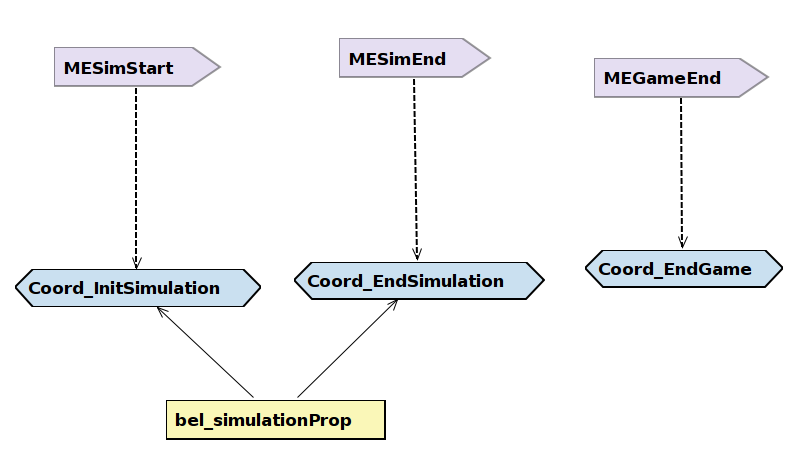
\includegraphics[scale=0.35]{coordinator-design}
\end{center}
\caption{The overall design of a \texttt{Coordinator} agent.}
\label{fig:coordinator-design}
\end{figure}

\subsubsection*{Beliefs}
\begin{itemize}
% \item \texttt{CellEmpty} and \texttt{CellGold}: keep track of which cells
% are known to have obstacles and gold, respectively.

\item \texttt{SimulationProp}: stores some properties of the current simulation
being played.

% \item \texttt{PlayerPosition}: stores how many gold pieces the player is
% currently carrying.
\end{itemize}

% Again, Figure \ref{fig:design_beliefs} depicts all the beliefs used in the
% agent system.



\subsubsection*{Events}

The following events are all used to implement the communication between the players and the coordinator. That is, the following events are sent by the players to the coordinator, who then handles them by means of its own plans (see Figure \ref{fig:design_communication} for a graphical representation).

\begin{itemize}
% \item \texttt{EUpdateBel}: update the information on some group for cells.

\item \texttt{MESimStart}, \texttt{MESimEnd}, and \texttt{MEGameEnd}: as described above to signal the start and end of simulations/games.

\end{itemize}




\subsubsection*{Plans}

The following plans are all used to handle events that were sent by the players:

\begin{itemize}
\item \texttt{Coord\_InitSimulation} and \texttt{Coord\_EndSimulation}: perform tasks associated to the start and end of simulations (e.g., initializing or resetting beliefset \texttt{SimulationProp}.

\item \texttt{Coord\_EndGame}: performs tasks associated to the end of a complete tournament game.

% \item \texttt{UpdateBeliefs}: updates the information about a group of cells
% in the grid.
\end{itemize}













%%%%%%%%%%%%%%%%%%%%%%%%%%%%%%%%%%%%%%%%%%%%%%%%%%%%
\section{System Operation Overview}
%%%%%%%%%%%%%%%%%%%%%%%%%%%%%%%%%%%%%%%%%%%%%%%%%%%%


\subsubsection*{System initialisation}

Initially, the agent connects to the game simulator and authenticates itself
using its login and password:
\begin{enumerate}
 \item The agent's \texttt{ClimaTalking} capability opens a socket
connection to the game server.

\item As soon as the player is created, a \texttt{EStart} event is 
automatically
posted.

\item Event \texttt{EStart} is handled by plan \texttt{AuthenticateToServer},
which in turn posts a \texttt{TellClimaServer} event with an
\texttt{AuthRequest} object as data containing the authentication information
obtained from the command line (i.e., login and password).

\item Finally, the \texttt{ClimaTalking} capability handles the event
\texttt{TellClimaServer} by sending corresponding XML authentication message to
the game server with the player details.
\end{enumerate}


At this point, the agent is connected and registered to the game
server. If for any reason the connection drops, the \texttt{ClimaTalking}
capability will automatically retry to connect and authenticate. Thus
the \texttt{ClimaTalking} capability maintains a robust permanent connection
with the game server.


\begin{figure}[t]
\begin{center}
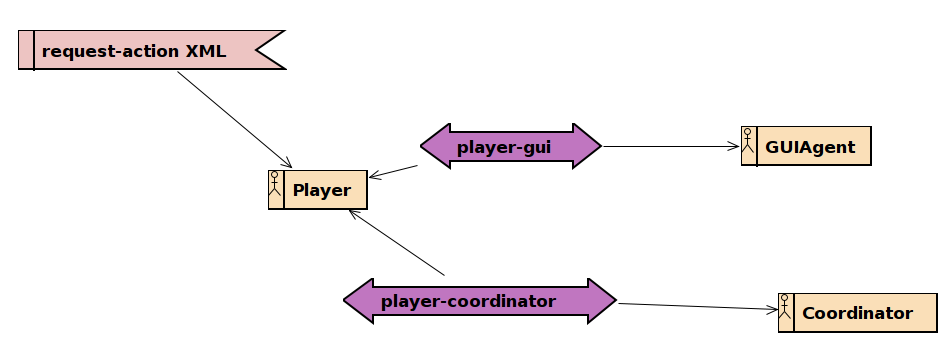
\includegraphics[scale=0.4]{agent-comm}
\end{center}
\caption{An overview of the agent communication.}
\label{fig:design_communication}
\end{figure}

\subsubsection*{Start of a new simulation}

Once the agent has successfully authenticates to the game server, it just waits
for a simulation to start. The start of a simulation happens as follows:
%
\begin{enumerate}
 \item The game server sends an XML \texttt{sim-start} message to the
agent.

 \item The \texttt{ClimaTalking} capability reads such XML message and posts a
\texttt{PerceiveClimaServer} event, whose data contains a \texttt{SimStart}
object.

\item The pending \texttt{PerceiveClimaServer} event is then handled by
the player's \texttt{StartSimulation} plan, which in turn sends an
\texttt{MESimStart} event to the coordinator agent.

\item The coordinator handles the \texttt{MESimStart} event using its plan
\texttt{Coord\_InitSimulation}.
\end{enumerate}


\subsubsection*{Playing a simulation game}

Once a simulation has started, it follows the following pattern:
%
\begin{enumerate}
 \item Agent receives a \texttt{request-action} as a
\texttt{PerceiveClimaServer} event that is posted automatically by the agent
\texttt{ClimaTalking} capability (see Section \ref{sec:clima-talking}).

\item Plan \texttt{HandlePercept} then handles such event by doing
the following:
%
\begin{enumerate}
\item Explicitly update part of the agent beliefs (e.g., number of gold being
carried, current position, simulation step number, etc.)

\item Post, synchronously,  an event \texttt{EUpdateBel} so that the agent
can further update its beliefs about the surrounding cells.

% \item Send the same event \texttt{UpdateBel} to the coordinator agent so as to
% share some information with it

\item Post, asynchronously, an event \texttt{EAct} to signal the need to select
and perform some action on the game server.

\item Post, asynchronously, an event \texttt{EShowBeliefs} so that the agent reports on its current state of affairs.

\end{enumerate}
\item The agent handles event \texttt{EUpdateBel} using its plan \texttt{UpdateCellArround}, which shall update the beliefs about the cell around the agent current location.

% \item The coordinator then handles event \texttt{UpdateBel} by means of its
% plan \texttt{UpdateBeliefs}

\item The agent will handle event \texttt{EShowBeliefs} using plans \texttt{ConsoleBeliefPrinting} and \texttt{BeliefPrinting}. For reporting anything on the console, one should use the first one.


\item The agent will handle event \texttt{EAct} using plan \texttt{MoveRandomly}
\end{enumerate}

Figure \ref{fig:design_simcycle} depicts the interaction between the different parts of the system that are involved in an agent playing a simulation game.


\begin{figure}
\begin{center}
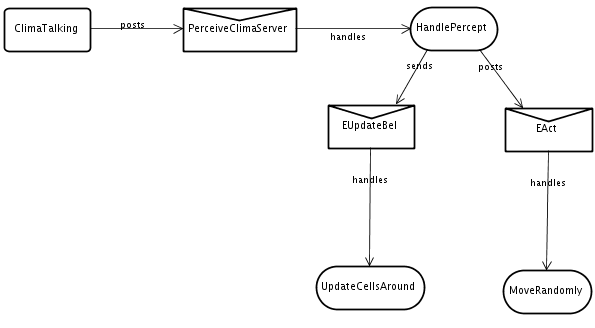
\includegraphics[width=12cm]{PlayerSimCycle}
\end{center}
\caption{An overview of the player interaction within a simulation.}
\label{fig:design_simcycle}
\end{figure}



\subsubsection*{End of a simulation}

The above process continues throughout the simulation until this is over, in which case the following occurs:

\begin{enumerate}
 \item The game server sends an XML \texttt{sim-end} message to the agent.
 \item The agent's \texttt{ClimaTalking} capability reads the XML message
	and posts a corresponding \texttt{PerceiveClimaServer} event, whose
	data contains an \texttt{MESimEnd}.

\item The pending \texttt{PerceiveClimaServer} event is then hanlded by plan
\texttt{FinishSimulation}, which in turn sends an \texttt{MESimEnd} event to the
coordinator agent

\item The coordinator would handle the \texttt{MESimEnd} event by means of plan
\texttt{Coord\_EndSimulation}.
\end{enumerate}

Once the simulation is over, the players came back to their ``waiting'' state
for a new simulation or the end of the whole tournament.


\subsubsection*{End of tournament}

Eventually, all the scheduled simulations were carried on by the server and the
complete tournament is over. In that case, the following occurs:

\begin{enumerate}
 \item The game server sends an XML \texttt{bye} message to the
player agent.

\item The agent's \texttt{ClimaTalking} capability reads the XML message 
and posts a corresponding \texttt{PerceiveClimaServer} event, whose data
contains a \texttt{Bye} object. Moreover, the capability disconnects completely
from the game server by closing the corresponding socket.


\item The pending \texttt{PerceiveClimaServer} event is then hanlded by plan
\texttt{FinishGame}. The plan basically may do some routine tasks and finally
terminate the agent by calling the agent base method \texttt{finish()}. Before
terminating, it informs the coordinator of the end of the tournament by sending
it an \texttt{MEGameEnd} event.

\item The coordinator then handles the \texttt{MEGameEnd} event by means of
plan \texttt{Coord\_EndGame}. This plan will also terminate the coordinator
agent, maybe after doing some routine tasks.
\end{enumerate}



%%%%%%%%%%%%%%%%%%%%%%%%%%%%%%%%%%%%%%%%%%%%%%%%%%%%
\section{Connectivity Infrastructure: The \texttt{Climma-Talking} Capability}
\label{sec:clima-talking}
%%%%%%%%%%%%%%%%%%%%%%%%%%%%%%%%%%%%%%%%%%%%%%%%%%%%

\begin{figure}
\begin{center}
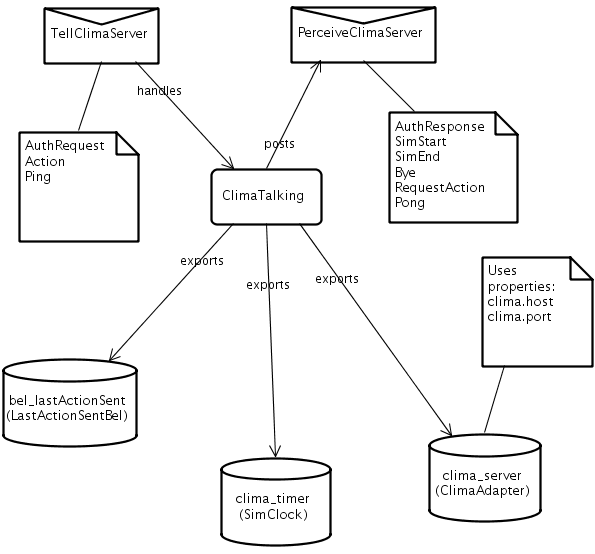
\includegraphics[width=8cm]{ClimaTalking_usage}
\end{center}
\caption{A usage view of the \texttt{ClimaTalking} capability.}
\label{fig:design_climatalking}
\end{figure}

The support infrastructure containing the connectivity code is wrapped up into a
single \texttt{ClimaTalking} \textit{capability}
(\texttt{rmit.ai.clima.iface.ClimaTalking}).
%
An overview of this capability is depicted in
Figure \ref{fig:design_climatalking}.
%
This capability is already included in the agent as an \textit{imported
external} entity, and thus it \textit{cannot} be modified within the
agent. The binary of the capability is included in JAR file
\texttt{lib/climacomms.jar}. To successfully compile the \JACK\ agent system, it
is necessary to have such JAR file within the CLASSPATH. 
% 
% If compiling within \JDE, the JAR file has to be added to the \textit{Project
% Classpath} option within the \textit{Compiler Utility}.





Before going into the details of the capability, it is worth noting that the
agent programmer should be able to develop a full agent system for the 
game \textit{without knowing almost any details about the capability}.
%
Understanding the two events \texttt{TellClimaServer} and
\texttt{PerceiveClimaServer}, together with the classes used to represent each
XML message (see below), should be enough to successfully develop an agent.
%
Figure \ref{fig:design_serverinteraction} shows how the player interacts with
the game server by either authenticating itself at connection time or sending
domain actions during simulation games.


\begin{figure}
\begin{center}
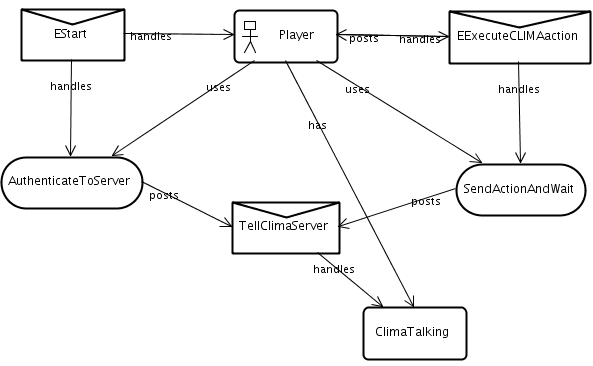
\includegraphics[width=10cm]{ServerInteraction}
\end{center}
\caption{An overview of the player interaction with the game server.}
\label{fig:design_serverinteraction}
\end{figure}


The \texttt{ClimaTalking} capability has the following four dynamic elements
(two event types and two data):
\begin{enumerate}
 \item The \texttt{TellClimaServer} event type
(\texttt{rmit.ai.clima.iface.TellClimaServer}), to issue messages to the
game server.

\item The \texttt{PerceiveClimaServer} event type 
(\texttt{rmit.ai.clima.iface.PerceiveClimaServer}), to carry received messages
from the game server.


\item The \texttt{ClimaAdapter clima\_server} data
(\texttt{rmit.ai.clima.iface.ClimaAdapter}), containing the low-level
settings and functions implementing the game server interactions.

\item The \texttt{SimClock clima\_timer} data
(\texttt{aos.jack.jak.util.timer.SimClock}), to keep the simulation time
provided by the game server.

\item The \texttt{LastActionSentBel bel\_lastActionSent\_dat} belief data to
keep the last ``id'' number of the action sent to the game server
(\texttt{rmit.ai.clima.iface.LastActionSentBel}). 
\end{enumerate}

The game messages (e.g., \texttt{SIM-START}, \texttt{REQUEST-ACTION},
\texttt{ACTION}, etc.) are all modeled as JACOB\footnote{Information on
JACOB can be found in the \JACK\ manual.} objects, and the above two events
\texttt{TellClimaServer} and  \texttt{PerceiveClimaServer} carry these as
data. 
%
This means that each particular  XML messages exchanged between the agent
and the game server will be eventually seen by your agents as a mere
JAVA object. The (JACOB) classes of those objects, which are already fully
defined, correspond one-to-one with the XML messages as documented
in file \texttt{c7c-protocol.txt}, except for trivial name renaming (e.g.
\texttt{RequestAction} instead of \texttt{REQUEST-ACTION}).




Note that the ClimaTalking capability makes use of Java properties for
connection  information. These are:
\begin{itemize}
\item {\bf clima.host} The host name of the Agent Contest
Server. (e.g., \texttt{yallara.cs.rmit.edu.au})
\item {\bf clima.port} The port name for client connections.
\end{itemize} (We will advertise a range of port numbers you can use
when running and testing).

The agent needs to provide the following for authorisation:
\begin{description}
\item[clima.agent.name.username] The authorization user name for
the agent named \textbf{name}.
\item[clima.agent.name.password] The authorization password for
the agent named \textbf{name}.
\end{description}
%
For initial experimentation you can use \texttt{participant1,
participant2, ..., participant6} and \texttt{1, 2, ... , 4, 5,
6} as agent names and passwords.\footnote{If you want to run 2
teams, you can also use the dummy \texttt{botagent} team that comes with the
game server.}
%
For the competition, we shall assign agent and password names.

The \texttt{ClimaTalking} capability is at the core of the connectivity
infrastructure. It deals with the sub-functions \nolinebreak of:
\begin{enumerate}
\item keeping a TCP connection with the game server, including the
authorisation hand-shaking with the game server;

\item parsing of incoming messages, translating them into their corresponding
JACOB objects, and then posting \texttt{PerceiveClimaServer} events
carrying the data;

\item handling \texttt{TellClimaServer} events by encoding their JACOB messages
into their corresponding XML messages, and sending them to the game
server; and

\item maintaining the \texttt{clima\_timer} time value, by peeping at the time
stamps of receive messages.


\item maintaining the \texttt{bel\_lastActionSent\_dat} id value, by storing the
id number of the last action sent to the game server (when the agent posted a
\texttt{TellClimaServer} event).
\end{enumerate}


The \texttt{ClimaTalking} capability is already included in the initial agent
so all connection and all low-level communication with the game server is
already included with it.


\subsection{XML Messages as JACOB Objects}

The \texttt{ClimaTalking} capability of each agent is in charge of doing the
low-level exchange of XML messages throughout the tournament. Outside this
capability, these messages are not seen as XML messages anymore, but as JACOB
objects.
%
There is one class defined for each possible XML messages in the domain.
The main events \texttt{TellClimaServer} and \texttt{PerceiveClimaServer} are
designed to carry on objects of these classes as their data.

A \texttt{TellClimaServer} event can carry, as its data, an object of any of
these classes: \texttt{AuthRequest}, \texttt{Action}, or \texttt{Ping}. 
%
Similarly, a \texttt{PerceiveClimaServer} event can carry as data an object of
any of the following classes: \texttt{AuthResponse}, \texttt{SimStart},
\texttt{SimEnd}, \texttt{Bye}, \texttt{RequestAction}, and \texttt{Pong}.

Probably the most sophisticated and important class is
\texttt{RequestAction}, corresponding to a \texttt{request-action} XML
message sent by the game server at every step of the simulation. Apart from
some basic information (e.g., the step number, the agent's current position,
etc.) an object of that class includes an attribute that is an array of an
auxiliary \texttt{Cell} class. Each object of class \texttt{Cell} would then
contain the particular information of a cell.

All these classes are defined within the \texttt{ClimaTalking} capability in
the package \texttt{rmit.ai.clima.comms}. So, for example, if an agent plan
needs to access some \texttt{SimStart} object (e.g., to extract the position of
the depot), it needs to import \texttt{rmit.ai.clima.comms.RequestAction}.

Finally, we point out that one can easily extract the form of each of these
classes (i.e., their attributes and methods) by inspecting file
\texttt{rmit/ai/clima/comms/msg.api}. As it is easy to observe, the attributes
of each class correspond one-to-one to the data contained in the corresponding
XML message, as dictated by the protocol.



%%%%%%%%%%%%%%%%%%%%%%%%%%%%%%%%%%%%%%%%%%%%%%%%%%%%
\section{The \texttt{gui.jar} Package}
%%%%%%%%%%%%%%%%%%%%%%%%%%%%%%%%%%%%%%%%%%%%%%%%%%%%

The \texttt{lib/gui.jar} file implements the graphical interface for the game. Besides providing such functionalities, used by agent \texttt{GUIAgent}, it the following useful libraries/packages:
%
\begin{itemize}
\item The actual GUI Window Java-based interface (class \texttt{GuiInterface}), within package \texttt{rmit.ai.clima.gui}.

\item Java interfaces used in the application, in package \texttt{rmit.ai.clima.interfaces}.

\item Class \texttt{GridPoint} in package \texttt{rmit.ai.clima.gui.grid} to manipulate points/cells \texttt{(x,y)} in the grid. It contains several utilities, some static, to manipulate cells in a convenient way (e.g., getting a cell as a String or calculating a cell adjacent to another one). Please refer to \texttt{GridPoint.java} to see what the class provides.

\item Class \texttt{GameGraphic} in package \texttt{rmit.ai.clima.gui.graphic} providing different graphical shapes (e.g., circles, rectangles, etc.) to represent different objects (e.g., gold, agents, obstacles, etc.).
%%
The agent system defines static graphical objects that will be used to represent different entities in the game in class \texttt{GameGraphics} within package \texttt{rmit.ai.clima.gui.grid}. This class also provides a convenient mapping between such graphical objects and string representations (e.g., ``gold'').
\end{itemize}






\subsection*{Acknowledgments}

We acknowledge the help of Ralph Ronnquist in developing the initial version of the \texttt{ClimaTalking} capability and providing support on many issues. 
%%
Phil Donald developed a first prototype of the GUI interface. 
%%
The current version of the GUI interface is due to Abhijeet Anand.
%%
We also thank Nitin Yadav for providing substantial support across the whole project.


% \bibliography{bibtea}
%\bibliographystyle{alpha}  % Others Styles:plain, unsrt, alpha, rv 
%\newpage % New page for the Appendix 
%\appendix
\end{document} 
%%%%%%%%%%%%%%%%%%%%%%%%%%%%%%%%%%%%%%%%%%%%%%%%%%%%%%%%%%%%%%%%%%%%%%%%%%%%%%
% EOF: aose-project06.tex
%%%%%%%%%%%%%%%%%%%%%%%%%%%%%%%%%%%%%%%%%%%%%%%%%%%%%%%%%%%%%%%%%%%%%%%%%%%%%%
